%%% 05-06-2015 updated from 30-04-2015 updated from 02-15-2015
%%% ONLY node and set of nodes robustness measure 
\documentclass[english,graybox]{svmult}
\usepackage[hang]{footmisc}
%\pagenumbering{arabic}
\setlength{\footnotemargin}{0pt}
\usepackage{footmisc,multicol, graphicx,makeidx,courier,helvet}
\usepackage[T1]{fontenc}
\usepackage[]{inputenc}
\usepackage{amssymb,amsmath} 
\usepackage{amsfonts}
\usepackage{booktabs}
\usepackage{subfigure}
\usepackage{graphicx}
\usepackage{epstopdf}
\usepackage{babel}
\newcommand*{\addheight}[2][.5ex]{%
\raisebox{0pt}[\dimexpr\height+(#1)\relax]{#2}%
}
\usepackage{mathptmx}         % selects Times Roman as basic font
\usepackage{helvet}         % selects Helvetica as sans-serif font
\usepackage{courier}        % selects Courier as typewriter font
\usepackage{type1cm}        % activate if the above 3 fonts are
\usepackage{makeidx}         % allows index generation
\usepackage{graphicx}        % standard LaTeX graphics tool
\usepackage{multicol}        % used for the two-column index
\usepackage{array}
\usepackage{tabularx}
\usepackage{caption}

\makeindex   

\begin{document}
\def\s{\sigma}

%\title*{An informational approach to the Network Disease Hypothesis in resting state fMRI}
\title*{Network efficiency as a classifier for aging in resting
state fMRI}
\author{Jaime Gomez-Ramirez, Yujie Li, Qiong Wu, Xiaoyu Tang, Jinglong Wu}
\institute{Biomedical Engineering Laboratory, Okayama University,  Japan}
%{   Biomedical Engineering Laboratory, Okayama University,  Japan
%\\ Autonomous Systems Laboratory, Universidad Polit�cnica de Madrid, %Spain \\
%{jd.gomez@upm.es}}
 
\maketitle

\abstract{Here we study network robustness i.e., resilience to
perturbations, in resting state functional connectivity networks (R-fMRI). We investigate the effect of the lesioning of indiviudual brain regions and networks of regions in young and elder subjects. We apply analytic measures of network communication efficiency in the human brain to make reasonable guesses about  compensatory mechanisms elicited in aging. 

}
\keywords{resting state fMRI, network degeneration hypothesis, Markov chain,
relative entropy}

\section{Introduction}
%The objective of this work is to study network robustness i.e., resilience to
%perturbations, in resting state functional connectivity networks.
%i.Relevance of RS 
It has been suggested that fluctuations in the BOLD signal measured
in humans in resting state, represent the neuronal activity baseline and shape
spatially consistent patterns \cite{Raichle:2005}, \cite{Fransson:2006}. The 
slow fluctuations in the BOLD signal found in resting subjects are highly
coherent within either structural or functional networks in the human brain.
%Therefore,
%exploring these fluctuations could lead to a better understanding of the
%brain's intrinsic or spontaneous neural activity. %i.But I dont help in this direction in this paper, delete this sentence?
Functional correlation based on the synchrony of low-frequency blood flow
fluctuations in resting state have been identified in the sensorimotor
\cite{kokkonen_preoperative_2009}, visual \cite{damoiseaux_consistent_2006},
language \cite{hampson_detection_2002}, auditory
\cite{hunter_neural_2006} and attention
\cite{fox_spontaneous_2006} and the frontoparietal control system
\cite{vincent_evidence_2008}.

%ii.Approaches 
The visual identification of the
overall connectivity patters in resting state functional magnetic resonance
imaging (R-fMRI), has been assessed first and foremost using either model-based and model-free
approaches. In the former, statistical parametric maps of brain activation are
built upon voxel-wise analysis location \cite{biswal_functional_1995}.
While this approach has been successful in, for instance, 
the identification of motor networks \cite{robinson_resting_2009}, it shows important limitations when
the seed voxel cannot be easily identified \cite{maldjian_functional_2001}.  
For example, in brain areas with unclear boundaries i.e., cognitive networks involved in memory or self processing operations \cite{fingelkurts_persistent_2011}. 
Independent Component Analysis (ICA), on
the other hand, is a model-free approach that allows separating resting
fluctuations from other signal variations, resulting on a collection of spatial
maps, one for each independent component, that represent functionally relevant networks in the brain
\cite{calhoun_review_2009}.
%Bad sentence, improve style
While ICA has the advantage over model-free methods that it does not need to
assume a specific temporal model of correlation between regions of
interest, the functional relevance of the different components is, however,
computed relative to their resemblance to a number of networks, based on
criteria that are not easily formalized \cite{biswal_toward_2010}.

%Graph-based 3ra via 
A third approach, complementary to the other two, which is becoming of paramount importance is the network-based approach. Graph-based techniques provide new
insights into the structure function relationship in the healthy brain, aging and neuropathological disorders \cite{fair_functional_2009}, 
\cite{wang_graph-based_2010}, \cite{he_graph_2010}, \cite{wang_graph_2011}, \cite{yu_altered_2011}, \cite{brier_functional_2014}, \cite{sala-llonch_changes_2014}. 
The use of graph theoretic techniques to model brain networks has shifted the 
emphasis from the identification of local subnetworks -default mode network,
primary sensory motor network etc.- to the quantitative study of the topological
and informational characteristics of large-scale brain networks.
Prove of the utility of this
approach is that notable proponents of a modularist vision of brain
connectivity to understand cognition, such as Gazzaniga
\cite{gazzaniga_new_1999} has
now embraced a complex brain networks approach \cite{bassett_understanding_2011}, \cite{Fuster:2000}.
%For an early critic of the
%modularist approach by Fuster contra Gazzaniga, see  )

Network-based approaches to R-fMRI data have demonstrated
non-trivial topological properties of functional networks in the human brain.
Large-scale anatomical
connectivity analysis in the mammalian brain, shows that brain topology is
neither random nor regular. Instead, small world
architectures \cite{Watts:1998} -highly clustered nodes connected thorough
relatively short paths- have been identified in brain networks. 
%\cite{Vaessen:2010}.
Small world networks are not solely
structural, functional networks with a small world organization have been
identified in the mammal brain \cite{Bassett:2006}. Small world network properties have also been consistently found across different
conditions, including normal development, aging, and
in various pathological conditions \cite{wang_graph-based_2010}, \cite{anderson_decreased_2013}, \cite{stam_modern_2014}. 
%http://www.ncbi.nlm.nih.gov/pmc/articles/PMC3604768/
While network-based studies have been successful in delineating generic network properties, such as
path length or clustering, additional work is needed in order to come to grips
with the internal working of the systems underlying the network.
Computational simulations of disruptions in the network
architecture of resting state can give clues about
normal development and pathological conditions. For example, Supekar and
colleagues \cite{Supekar:2008} have shown that the deterioration of small world
properties such as the lowering of the cluster coefficient, affect local
network connectivity, which in turn may work as a network biomarker for
Alzheimer's disease. Abnormalities in small-worldness may also have a
significant positive correlation in, for example, schizophrenia
\cite{liu_disrupted_2008} and epilepsy \cite{liao_altered_2010}, \cite{zhang_altered_2011}.

%Transport efficiency
Transport network efficiency measures have been used to study the relationsip between structural and resting state functional connectivity \cite{goni_resting-brain_2014}. 
The effects of lesioning in white matter connections can be studied via the simulation of the removal of individual connections from the connectome. Irimia and Van Hornreport \cite{irimia_systematic_2014}, using this technique have been able to delineate "a core scaffold" or white matter network connections that when disrupted, show dramatic changes in the overall organization of the human connectome.   
A systematic study of the effects of simulated lesioning in R-fMRI is still missing. Here we 
provide efficiency and robustness measures that show a more idiosyncratic response, in elder compared to young subjects, to brain region lesioning.
%We further demonstrate that MORE RESULTS  

The rest of the paper is structured as follows. Section \ref{mat-methods} introduces the 
methodology followed in the data acquisition and reconstruction, data
pre-processing, and data connectivity analysis in the young and elder conditions. Then, we build a model to study
quantitatively how network robustness is affected upon the removal of nodes in
the functional connectivity network in both conditions. We provide an efficiency loss metric  to quantify the impact of lesioning  based on \cite{latora_efficient_2001}.
The empirical and clinical implications of the theoretical model are described in the results section \ref{results}. 

\section{Materials and Methods}
\label{mat-methods}

%Materials Experimental (Li)
\subsection{Data acquisition}
Forty-two healthy volunteers separated in two groups, young (ages 21-32; mean
22.7) and elder (ages 51-59; mean
?) took part in the fMRI experiment. All subjects had
normal or corrected-to-normal vision. The study was approved by the ethics
committee of Okayama University, and written informed consent was obtained before the study. All subjects were imaged using a 1.5 T Philips scanner vision whole-body MRI system (Okayama University Hospital, Okayama, Japan), which was equipped with a head coil. Functional MR images were acquired during rest when subjects were
 instructed to keep their eyes closed and not to think of anything in
 particular. The imaging area consisted of 32 functional gradient-echo planar
 imaging (EPI) axial slices (voxel size=3x3x4 mm3, TR=3000 ms, TE=50 ms,
 FA=90�, 64x64 matrix) that were used to obtain T2*-weighted fMRI images in the
 axial plane. We obtained 176 functional volumes and excluded the first 4 scans
 from analysis. Before the EPI scan, a T1-weighted 3D magnetization-prepared
 rapid acquisition gradient echo (MP-RAGE) sequence was acquired (TR=2300 ms,
 TE=2.98 ms, TI=900 ms, voxel size=1x1x1 mm3).

\subsection{Data preprocessing} 
Data were preprocessed using Statistical Parametric Mapping software SPM8
\footnote{http://www.fil.ion.ucl.ac.uk/spm/} and REST v1.7
\footnote{http://restfmri.net/forum/index.php}. To correct for differences in
slice acquisition time, all images were synchronized to the middle slice.
Subsequently, images were spatially realigned to the first volume due to head
motion. None of the subjects had head movements exceeding 2.5 mm on any axis or
rotations greater than 2.5�. After the correction,  the imaging data were
normalized to the Montreal Neurological Institute (MNI) EPI template supplied
with SPM8 (resampled to 2x2x2 mm3 voxels) \footnote{http://imaging.mrc-cbu.cam.ac.uk/imaging/Templates}. In order to avoid
artificially introducing local spatial correlation, the normalized images were
not smoothed. Finally, the resulting data were temporally band-pass filtered
(0.01-0.08 Hz) to reduce the effects of low-frequency drifts and high-frequency
physiological noises \cite{jiao_granger_2011}.

\subsection{Anatomical parcellation} 
Before whole brain parcellation, several sources of spurious variance including
the estimated head motion parameters, the global brain signal and the average
time series in the cerebrospinal fluid and white matter regions were removed
from the data through linear regression. Then, the fMRI data
were parcellated into 90 regions using an automated anatomical labeling template (AAL) \cite{tzourio-mazoyer_automated_2002}.
For each subject, the mean time series of each region was obtained by simply
averaging the time series of all voxels within that region.

\subsection{Brain network construction} 
To measure the functional connectivity among regions, we calculated the Pearson
correlation coefficients between any possible pair of regional time series, and
then obtained a temporal correlation matrix $(90x90)$ for each subject. We
applied Fisher's r-to-z transformation to improve the normality of the
correlation matrix. Then, two-tailed one-sample t-tests were performed for all
the possible $4005=\frac{90x89}{2}$ pairwise correlations across subjects
to examine whether each inter-regional correlation significantly differed from
zero. 
A Bonferroni-corrected significance level of $p < 0.001$ was
further used to threshold the correlation matrix into an adjacency matrix whose
element was 1 if there was significant correlation between the two brain
regions and 0 otherwise. Finally, an undirected binary graph was acquired in
which nodes represent brain regions and edges represent links between regions.
%The study of the connectivity distribution of the resulting adjacency matrix is
%provided in the Appendix \ref{appendix}.


\subsection{Information Efficiency}
\label{ss:nrobeffvul}
%Distance related measures (Network Efficiency and Network Vulnerability)
A quantitative understanding of network robustness, that is, functional
network invariance under perturbation can shed light on 
the properties that mediate in developmental, aging and pathological processes
in the human brain. In essence, robustness measures the capacity of the network to
perform the same function before and after a perturbation. Perturbations are
events, internal or external, that elicit a change in the network
configuration. Possible perturbations are the obliteration of a node and a change in the
connectivity between nodes. Here we perform perturbations that consist on the obliteration of one or more nodes together with and all the edges that connect the lesioned node.
%Thus, for a given network $G(N,E)$ a perturbation consisting on the removal of a set of nodes $M$ from the initial set of nodes $N$, transforms
%the initial graph $G(N,E)$ into a new graph $G(N-M,E-E(M))$, where $N-M$ is the remaining
%set of nodes after having deleted the set $M$ and $E-E(M)$ is the set of edges
%that do not connect any of the deleted nodes in $M$ or $E(M)$. 
%The robustness of the new
%network $G(N-M,E-E(M))$ resulting of the perturbation $\delta$ can be studied
%as a loss in the network efficiency $\Sigma$ driven by the elimination of a set
%of nodes $M$ and the edges that connect them. 

The efficiency of a network is a network centrality
measure that quantifies the network's reliability in transmitting information once a
node or a set of nodes have being removed. One possible measure of network
efficiency is the 
Latora and Marchiori \cite{latora_efficient_2001} measure of network
efficiency defines the efficiency in transmitting information 
between any two nodes (i,j) in a graph G as the inverse of the shortest path that
connects them
\begin{equation}
\varepsilon_{ij}= \frac{1} {d_{ij}}
\label{eq:geod}
\end{equation}
where $d_{ij}$ is the
shortest path length or the geodesic distance between nodes $i$ and $j$. 
Note that when there is no path that connects the nodes i and j, $d_{ij}=
\infty$, and the efficiency in the communication of the two nodes is zero,
$\varepsilon_{ij}=0$.

The efficiency of the graph G, $\Sigma(G)$, is calculated as the average of the efficiency
between any two nodes $\varepsilon_{ij}$ 
\begin{equation}
\Sigma(G)=\frac{\sum_{i \neq j \in G} \varepsilon_{ij}} {N(N-1)}
=\frac{1}{N(N-1)}\frac{1}{\sum_{i \neq j \in G} d_{ij}}
\label{eq:latm}
\end{equation}
where $N$ is the number of nodes. 
 
We can calculate
the information centrality $C$ of any node i in a network G as the variation
in the network efficiency caused by the removal of the edges incident in i. Thus, the
centrality of a node i, $C_i$, is calculated as the difference between the
efficiency of the original graph G with N nodes and E edges, $G(N,E)$, and the
efficiency of the resulting graph $G(N,E-k_i)$ with N nodes and $E-k_i$ edges, where
$k_i$ denotes the set of edges incident to node i. The centrality of a
node is a normalized measure of the loss in network efficiency, caused by the isolation of a node in G.

\begin{equation}
C_i=\frac {\Sigma(G(N,E)) - \Sigma(G(N-i,E-k_i))} {\Sigma(G(N,E))} 
\label{eq:centr}
\end{equation}
From equation \ref{eq:centr}, a network $G$ is considered to be robust to
a perturbation $\delta$ if the network efficiency, $\Sigma(G)$, 
stays close to the original value after a perturbation. Ideally $\Sigma(G(N,E)) = \Sigma(G(N,E-k_i))$
with efficiency loss or centrality of node i equals to 0.
By the same token, the information centrality of a set of nodes $S$ or the efficiency loss upon the removal of $S$, can be
calculated as the normalized measure of the loss in network efficiency caused by the isolation of a set of nodes S in G
\begin{equation}
C_S=\frac {\Sigma(G(N,E)) - \Sigma(G(N-S,E-k_S)) } {\Sigma(G(N,E))} 
\label{eq:centrS}
\end{equation}

%%%%%%%%%%%%%%%%%%%%%%%%%%%%%%%%%%%%%%%%%
%%%%%%%%%%%%%%%%%%%%%%%%%%%%%%%%%%%%%%%%%
%%%%%%%%%%%%%%%%%%%%%%%%%%%%%%%%%%%%%%%%%
\section{Results}
\label{results}

% random 
In what follows we calculate, for both conditions, the network efficiency prior to any insult (Section \ref{ss:prior}), the efficiency loss after single node lesioning (Section \ref{ss:single}) and the efficiency loss after lesioning specific networks of interest (Section \ref{ss:target})
%Results

\subsection{Efficiency prior perturbation}
\label{ss:prior}
%1. uperturbed
 The global network efficiency for unperturbed networks as defined in Equation \ref{eq:latm} is
 0.3678 for young subjects and 0.1144 for elder subjects. Thus, young subjects
 connectivity network is a bit more than three times (3.21) more efficient in terms of the shortest
 path distance between any two nodes. The 
 the number of edges in the young condition is 718 and in the young condition is 308, the average degree connectivity are 8.97 and 4.42 respectively \ref{fig:adjmat}.
 
 %i adjacency matrix both y and o
%%%%%%%%%%%%%%%%%%%%%%%%%%%%%%%%%%%%%%%%%%%%%%%%%

\begin{figure}[!ht]
    \subfigure[\label{subfig-1:dummy}]{%
      \includegraphics[width=0.5\textwidth,height=0.5\textheight,keepaspectratio]{figures/youngadjmatrix.pdf}
    }
    \hfill
    \subfigure[\label{subfig-2:dummy}]{%
      \includegraphics[width=0.515\textwidth,height=0.515\textheight,keepaspectratio]{figures/oldadjmatrix.pdf}
    }
    \caption{\small (a) Adjacency matrix in the young condition.   
  \small (b) Adjacency matrix old condition. The red dots prepresent connections between two nodes. In the old condition the adjacency matrix is more sparse, it has 308 edges (718 edges in the young condition)}
    \label{fig:adjmat}
  \end{figure} 
 
 
%2.perturbation analysis. Random random 1 node deletion

\subsection{Efficiency after single node lesioning}
\label{ss:single}
In order to obtain the efficiency measures described in Equations \ref{eq:centr} and \ref{eq:centrS} we perturb the resting state network in two ways. First, using random node deletion and second targeting specific networks. In the random node deletion case, we build a population of networks perturbed by the systematic lesioning of single nodes. This is described next in Section \ref{sse:randomn}. In section \ref{sse:targetn} we target specific networks, that is, a number of networks of interest are lesioned and the efficiency loss calculated.
  
The population of perturbations $P$ that result from the systematic deletion of all nodes in all possible combinations, from an initial network of N nodes, has as many networks as  
\begin{equation*}
|P| = \sum_{i=1}^{N} C(N,i) = \frac{N!} {(i!)(N-i)!}
\label{eq:perurb}
\end{equation*}

For example, the population of networks that result from the deletion of one single node has 90 networks 
\begin{equation*}
\sum_{i=1}^{1}
C(90,i)_{i=1} = \frac{90!} {(1!)(90-1)!} = 90
\end{equation*}

Similarly, the number of perturbed networks obtained by deleting two nodes in all possible ways contains 4005 networks
\begin{equation*}
\sum_{i=1}^{2} C(90,i)_{i=2} =
 \frac{90!} {(2!)(90-2)!} = 4005
\end{equation*}

We build a distribution of the efficiency measures described in section \ref{eq:latm}
for both young and elder condition for the systematic removal of one node. Thus, in the young condition, we denote $P_{y, 90}$ the distribution of networks with only one node removed, that is, $P_{y, 90}$ has 90 different networks where for each one a node and its connections have been deleted. 
The mean of the efficiency measure for $P_{y, 90}$ is 0.358. The removal of node  "Inferior temporal gyrus" (89) has no effect in the efficiency, that is, the network efficiency before and after the removal has identical value. 
Nodes 35 and 36 ("Posterior cingulate gyrus") have also an extremely mild effect after their removal. The most significant loss in efficiency occurs with the removal of node 74 ("Lenticular nucleus, putamen") followed by node 31 ("Insula right") (Figure \ref{fig:boxplot}). 

The average efficiency loss in the young condition is $2.44"\%" $ with a maximum of  $4.67"\%" $ for node 74 ("Lenticular nucleus, putamen") and no efficiency loss for node 89 ("mporal pole: middle temporal gyrus"). The rationale for the different impact in the efficiency caused by the obliteration of certain nodes can be found in the connectivity degree. In general, the nodes that after their removal trigger a low efficiency loss have also low connectivity degree and those that produce a more pronounced reduction of the network efficiency tend to be more connected (Figure \ref{fig:gauss}). 

Similarly, for the elder condition, we denote $P_{o, 90}$ the distribution of networks with only one node removed in the elder condition. 
The mean of the efficiency measure (equation \ref{eq:latm}) for the 90 networks obtained upon single node deletion is $0.109$. As it happened in the young condition, the removal of node  "Inferior temporal gyrus" (89) has no effect in the efficiency, that is, the network efficiency before and after the removal of the "Inferior temporal gyrus" has identical value. 
Interestingly, the removal of nodes with the lowest connectivity degree (2) have also no quantifiable effect in the network efficiency (Figure \ref{fig:boxplot}). 
%33,39,63,71,73,75,77,78,80,85 

The most significant loss in efficiency occurs with the removal of node node 62 "Parietal Inf R". After the removal of this node, the efficiency loss relative to the original network is the $32.87"\%"$. This is an interesting result since node 62 is not a highly connected node, its connectivity degree is 6. Nodes 24, 44 and 51 have more connections, connectivity degree 10, and upon their deletion the efficiency loss is not as severe as in the case of node 62. 
The mean efficiency loss in the elder condition after the removal of a single node is  $4.61"\%"$. The effect in the loss of efficiency triggered by the disconnection of brain areas is more stereotypical in the elder condition than in young condition, that is, the connectivity degree is a much worse predictor of efficiency loss for old than for young (Figure \ref{fig:gauss}).
%node 24, 0.2892 and the other 2 really small node 44 0.0387, node 51 0.0382

\begin{figure}[!ht]
    \subfigure[Young: Efficiency after one node deletion\label{subfig-1:dummy}]{%
      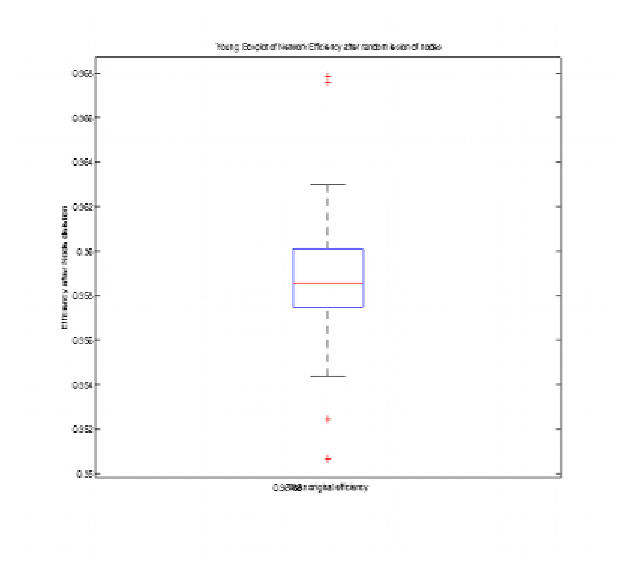
\includegraphics[width=0.55\textwidth,height=0.5\textheight,keepaspectratio]{figures/Fig-2-y-boxplot-eff_p.eps}
    }
    \hfill
    \subfigure[Old: Efficiency after one node deletion\label{subfig-2:dummy}]{%
      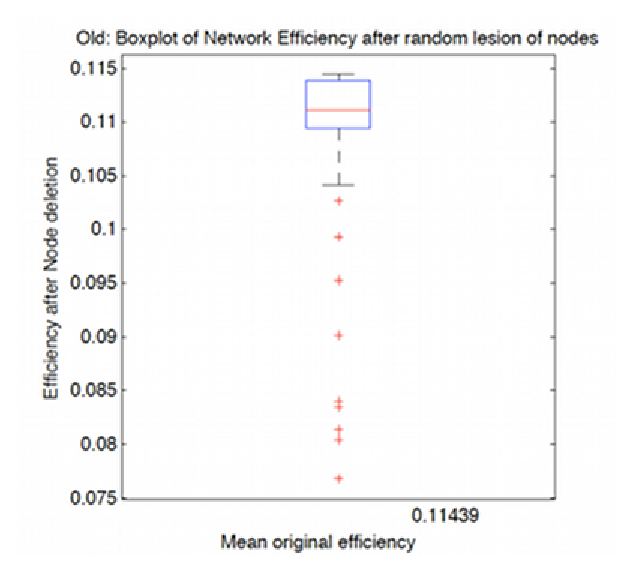
\includegraphics[width=0.525\textwidth,height=0.45\textheight,keepaspectratio]{figures/Fig-2-o-boxplot-eff_p.eps}
    }
     \subfigure[Young: Degree distribution (X) Efficiency loss (Y)\label{subfig-1:dummy}]{%
      \includegraphics[width=0.5\textwidth]{figures/regressionyoung.pdf}
    }
    \hfill
    \subfigure[Old: Degree distribution (X) Efficiency loss (Y)\label{subfig-2:dummy}]{%
      \includegraphics[width=0.49\textwidth]{figures/regressionold.pdf}
    }
    \caption{\small (a) Boxplot of network efficiency after random lesion of individual nodes. Only a very few nodes fall outside the box of the figure whose edges are the 25th and 75th percentiles. \small (b) Boxplot of network efficiency after random lesion of individual nodes. More nodes fall outside below the 25th percentile than in the young condition. The distribution in the elder condition is more skewed than in the young condition.\small (c) Degree distribution (x-axis) and efficiency loss (y-axis) after single node connectivity removal in the young condition.
  \small (d)  Degree distribution (x-axis) and efficiency loss (y-axis) after single node connectivity removal in the elder condition. The linear regression in the young condition is 0.755 and in the old condition is 0.4002. The effect in the loss of efficiency triggered by the disconnection of brain areas is more stereotypical in the elder condition than in young condition.}
    \label{fig:boxplot}
  \end{figure}


%\begin{table}[h]
%\begin{tabular}{cc}
%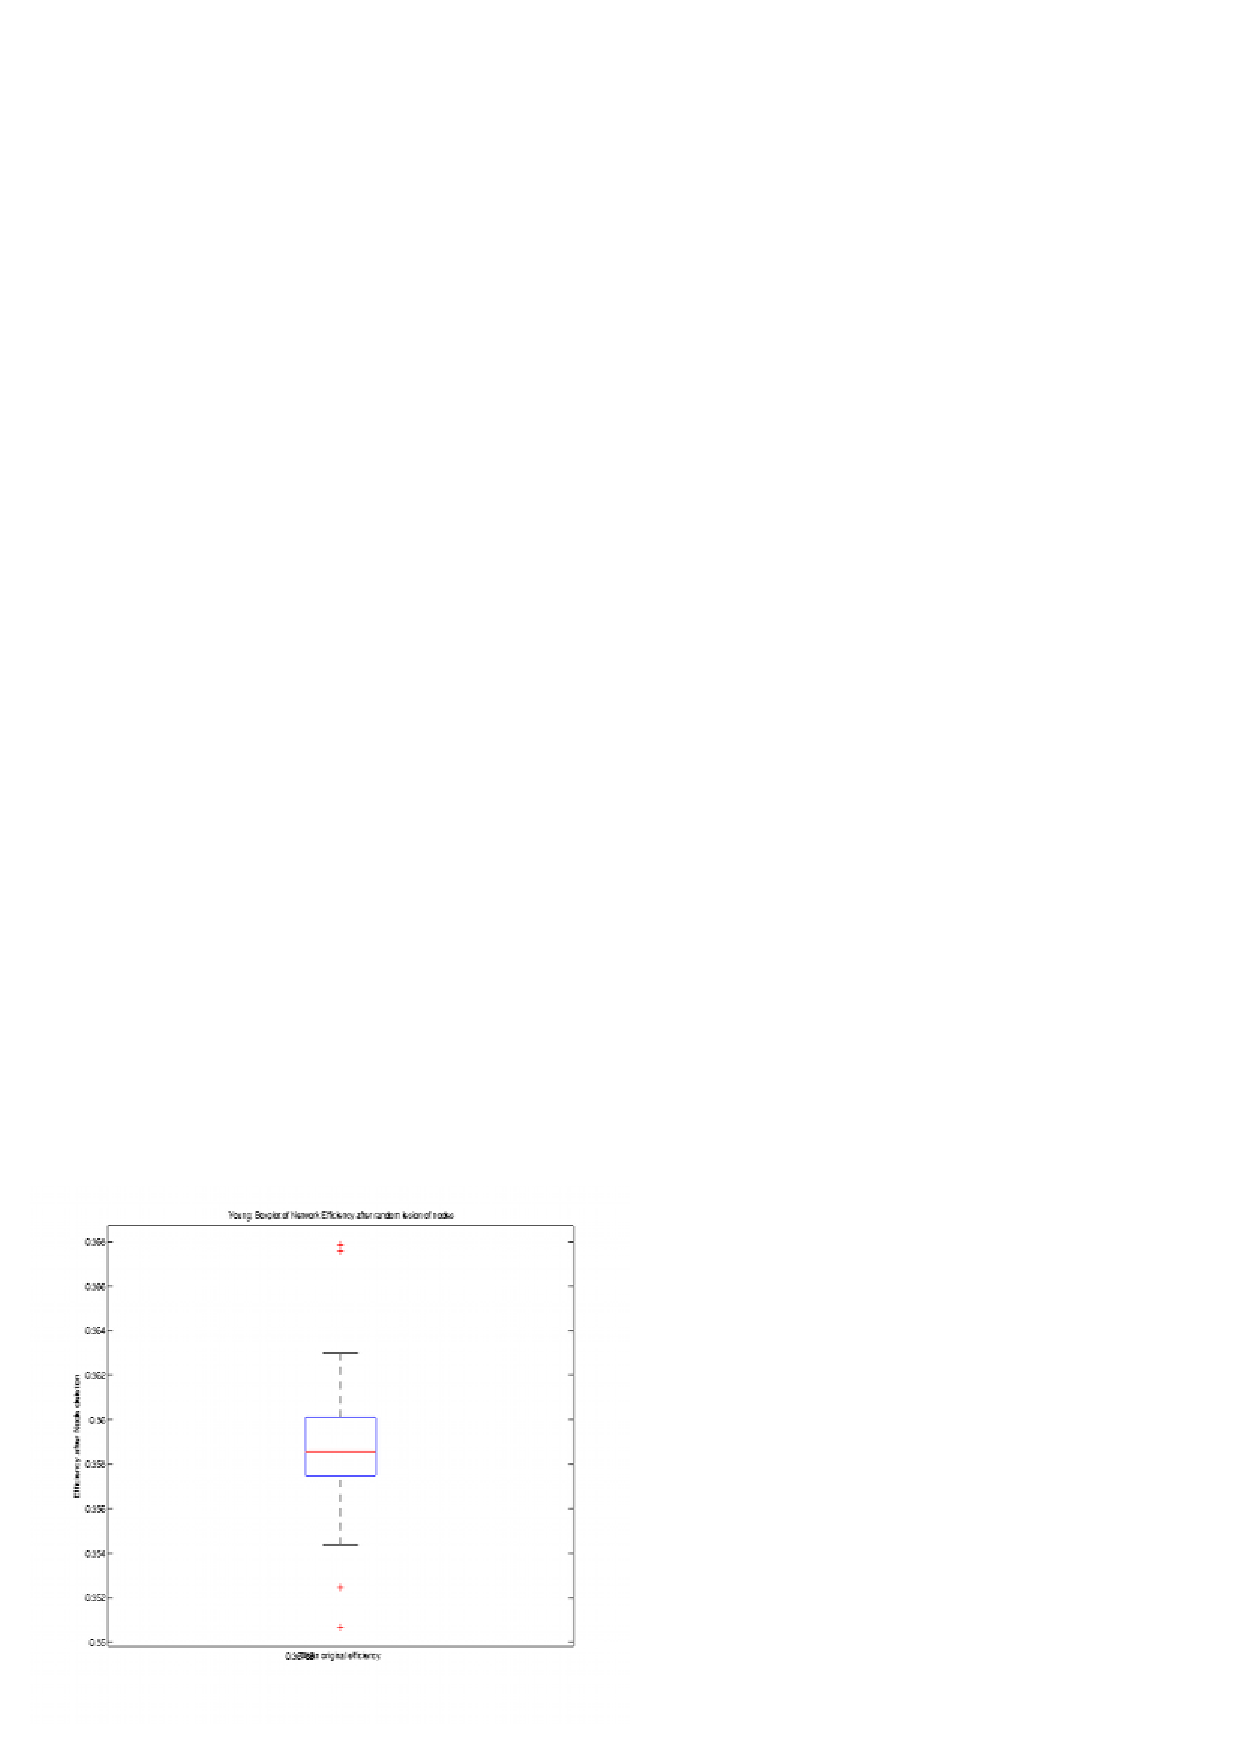
\includegraphics[height=2.5in]{figures/Fig-2-y-boxplot-eff_p.pdf}  \\ \small (a) \\ 
%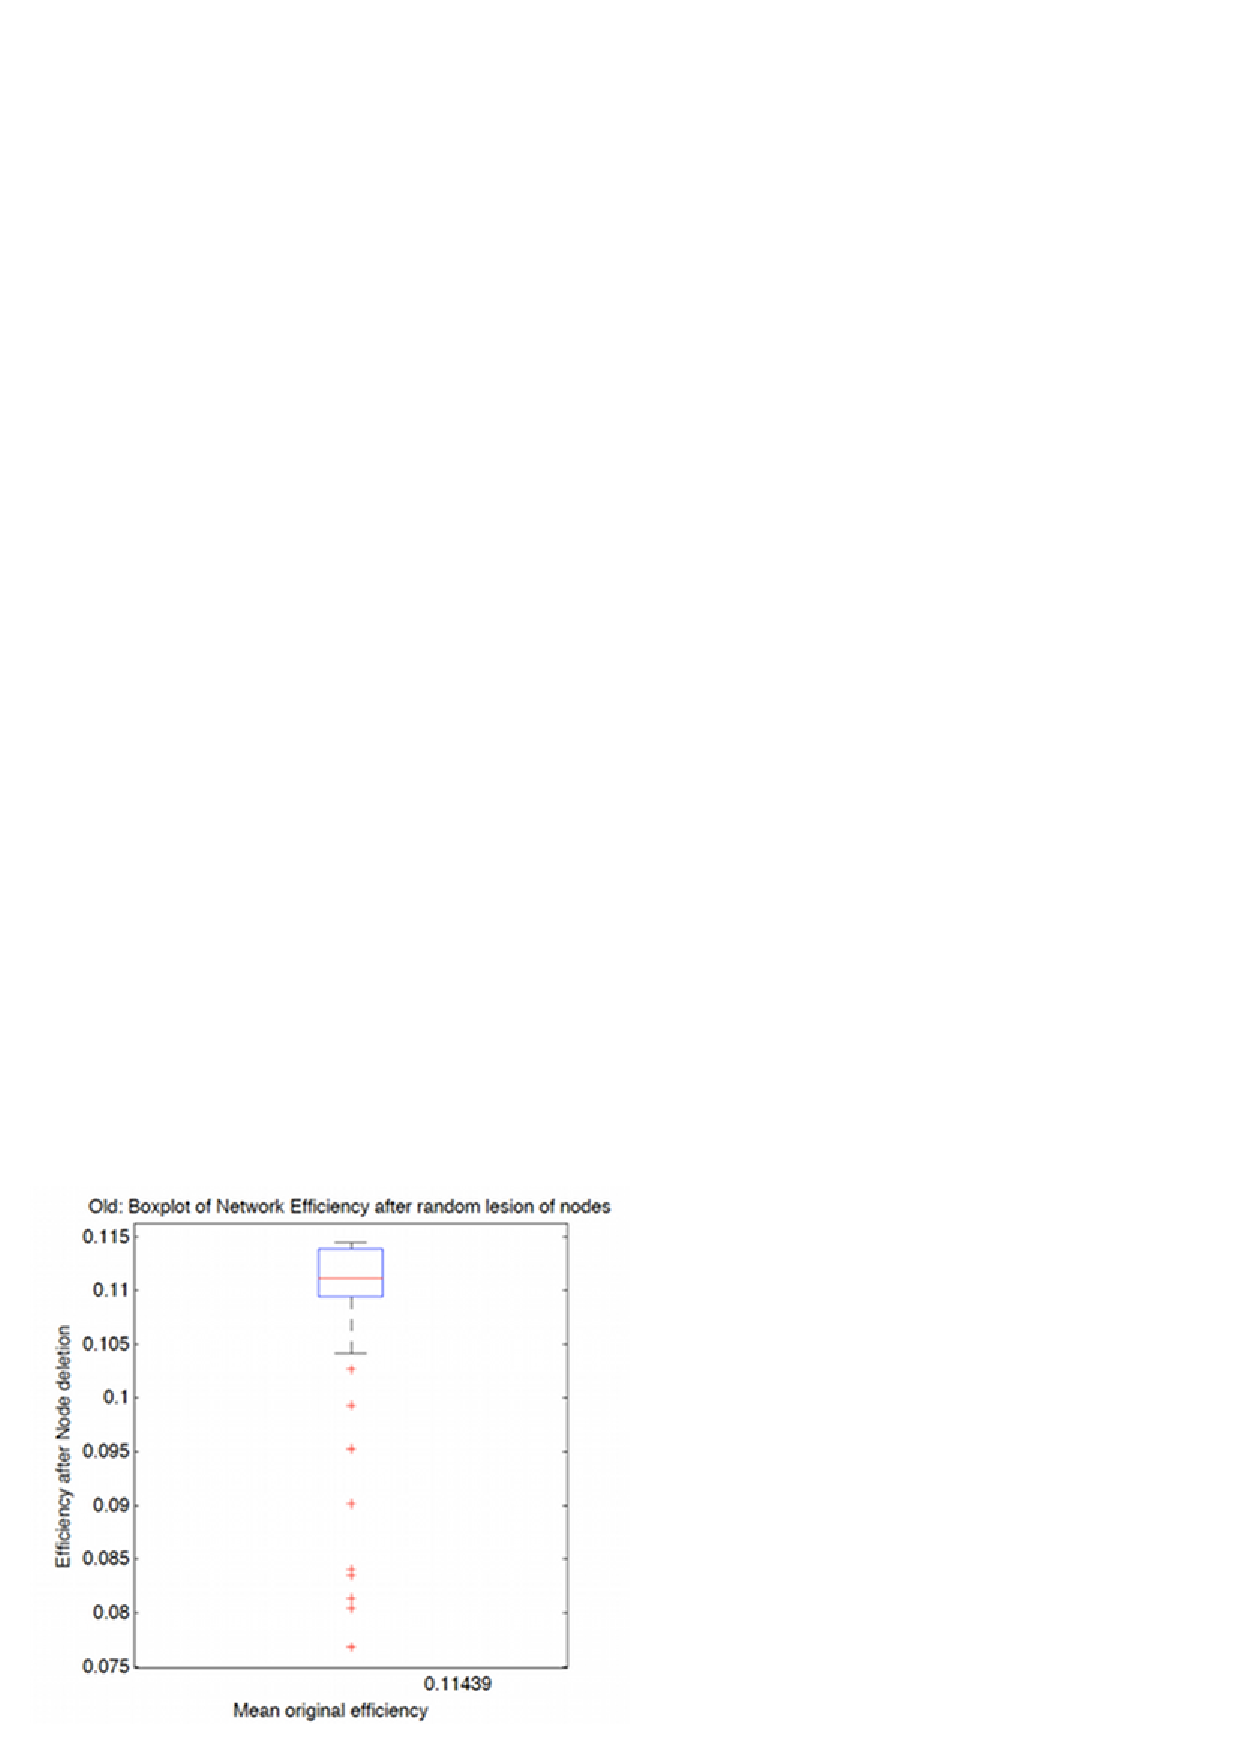
\includegraphics[height=2.5in]{figures/Fig-2-o-boxplot-eff_p.pdf} \\  \small (b)
%\end{tabular}
%\caption{
%\small (a) Boxplot of network efficiency after random lesion of individual nodes. Only a very few nodes fall outside the box of the figure whose edges are the 25th and 75th percentiles. \small (b) Boxplot of network efficiency after random lesion of individual nodes. More nodes fall outside below the 25th percentile than in the young condition. The distribution in the elder condition is more skewed than in the young condition.}
%\label{fig:box}
%\end{table}


\begin{figure}[!ht]
    \subfigure[Efficiency loss in young (blue) and old (red) for single node removal\label{subfig-1:dummy}]{%
      \includegraphics[width=0.51\textwidth,height=0.5\textheight,keepaspectratio]{figures/fig-4-eff-loss.pdf}
    }
    \hfill
    \subfigure[Frequency bars for efficiency loss in young (green) and old (blue) for single node removal\label{subfig-2:dummy}]{%
      \includegraphics[width=0.5\textwidth,height=0.5\textheight,keepaspectratio]{figures/lossdistrib-greenisYoung-blueisold.pdf}
    }
     
    \caption{\small (a) Efficiency loss normalized (0,1) due to the removal of each node in both elder and young condition. While in the young condition there are no nodes that upon its removal the efficiency of the resulting network drastically deteriorates, in the elder condition there are 6 nodes that upon their removal trigger a $20\%$ or more reduction in the  network efficiency. Nodes 8,$29.7\%$  24,$28.9\%$   34,$27.1\%$  56,$21.2\%$  62,$32.8\%$  64,$26.5\%$.   
  \small (b) Distribution of efficiency loss after node removal in both young (green histogram) and elder condition (blue histogram). The efficiency loss in the young condition is narrow. The elder condition, on the other hand, has a more spread distribution of efficiency values. 
The range in efficiency loss in the young condition varies a $4.67\%$ and in the elder condition varies a $32.87\%$}
    \label{fig:gauss}
  \end{figure} 
  
%%%%%scatterhit
%i
%\begin{figure}[!h]
%\begin{center}
%\centerline{\includegraphics [scale=0.3]  {figures/fig-3-scatterhist.pdf}}
%\caption{  Scatter histogram of young x-axis and old subjects, y-axis.}
%\label{Fig:scaterhist}
%\end{center}
%\end{figure}

\subsection{Efficiency after target networks lesioning}
\label{ss:target}

So far, we have quantified the efficiency loss due to the removal of single nodes, in what follows we investigate how efficiency is affected by removal of entire networks of interest. In particular we study the efficiency loss or centrality of nine different networks or brain structures, the Defaul Mode Network (DMN), Visual Network, temporal lobe, frontal lobe, insula and cingulate gyrus, occipital lobe, parietal lobe, central structures and limbic structures.
 
%%Hypothesis testing
The DMN is commonly considered to consist of medial prefrontal cortex
(AAL 23, 24, 25, 26), posterior cingulate cortex/precuneus (AAL 35, 36/67 68)
and bilateral inferior parietal lobule (AAL 61, 62). 
The removal of the DMN in
young adults triggers an efficiency loss of the $19.6\%$. In the elder condition, the same procedure yields an efficiency reduction of $61.66\%$. It ought to be remarked that the lesioning of the 10 AAL regions that compose the DMN network, which represents the $11\%$ of the total regions 90 regions, bring down the efficiency of the network to $61.66\%$.
%Figure DMN
The strong efficiency reduction associated with the lesioning of the DMN is coherent with the hypothesis that there is a decrease in activity in the DMN in aging. This age-based reduction in DMN activity can trigger  mechanisms that compensate the loss in DMN activity with an increase in connectivity between the DMN and other networks \cite{damoiseaux_reduced_2008}. According to this hypothesis, the DMN becomes a more central network and upon the lesioning of the DMN a larger efficiency loss is produced. 
We apply the efficiency measure for lesioning of edges and we we found no significant effect of age on DMN inter-connectivity ($0.16\%$ of efficiency loss in young subjects and $0.9\%$ in old subjects upon the disconnection of areas in different hemispheres). This result is in agreement with previous studies of aging on default mode network activity in resting state fMRI: \cite{koch_effects_2010} 

%- "The older subjects exhibited significantly lower DMN activity in the posterior cingulate (PCC, t-test P<.001) as well as a tendency to lower activity in all other DMN regions in comparison to the younger subjects. TEST this: We found no significant effect of age on DMN inter-connectivity."
%http://www.ncbi.nlm.nih.gov/pubmed/20004726



%http://www.ncbi.nlm.nih.gov/pmc/articles/PMC4392680/
The vision-related brain regions (hereafter called Visual) in the AAL template include left and right calcarine fissure and surrounding cortex (Nodes 45,46), left and right lingual gyrus (Nodes 47,49), left and right superior occipital gyrus (Noes 49,50), left and right middle occipital gyrus (Nodes 51, 52), left and right inferior occipital gyrus (Nodes 53, 54), left and right fusiform gyrus (Nodes 55, 56), left and right superior parietal gyrus (Nodes 59,60), and right inferior temporal gyrus (Nodes 89, 90). The removal of the Visual network in young adults triggers an efficiency loss of the $38.93\%$ while in the elder condition the same procedure yields a $55.98\%$.
 
 
\subsection{Efficiency after target networks lesioning of edges}
\label{ss:edges}
  
\section{Discussion}
\label{discussion}

We have analyzed the functional connectivity in resting state of both young and
elder individuals, using a perturbational approach consisting on either the systematic removal of single nodes and the removal of entire networks of interest such as the DMN and others. We have computed the loss in network efficiency upon the lesioning of brain areas.
%Random removal 1 node
Our results expand previous works on the study of robustness of
structural brain networks. %
Interestingly, we find that the distribution of network efficiency in the young and the elder condition show very different signatures. The functional resting state network in young adults is more robust to node removal than in elder subjects. The efficiency loss in young subjects, upon the removal of single nodes, is always below the $5\%$ while in the elder condition the removal of individual nodes may yield a dramatic reduction of the network efficiency.
The young adults are, thus, more robust to random deletion of single nodes nodes. However, when the lesioning is focused in specific brain networks rather than single regions, the efficiency loss for young subjects is in occassion higher than when the same damage is done in old subjects. For example, the disconnection of the occipital lobe, limbic structures and central structures yield  a larger efficiency loss in the young condition.     


%Hypothesis testing: SVM
In \cite{vergun_characterizing_2013} applied a Support Vector Machine (SVM) linear classifier to rs-fMRI data in order to compare age-related differences in four of the major functional brain networks: the default, cingulo-opercular, fronto-parietal, and sensorimotor. 
With this method they detected ?connectivity hubs,? or nodes with the most significant features that influenced age classification. The best redictors of age based on SVM are not coincident with the best predictors in age using the efficiency loss method.


%Hypothesis testing: Asymmtry
We test the asymmetry hypothesis by which brain activity shows a more balance activity among the two hemispheres with age, that is, the hypothesis predicts that in young individuals brain activity is more asymetric than in old indivduals. To test it we lesion sequentally the left and the right hemisphere and we calculate the efficiency loss for each case. In young individuals the difference in efficiency loss for disconnecting the hemispheres is expected to be larger than in the old condition. Aging thus, tries to compensate the reduction of   activity level, for example in the DMN, by balancing the activity accross the brain. 
%delete all odds, delete all even, Distance
We see, on the contrary, that if one of the two hemisphere is entirely lesioned, the efficiency loss in young adults is 0.7532 when the left side is lesioned and 0.7701 when the right side is gone. The difference is 0.0169.
In old sbjects, the lesioining of the right side has a more pronounced impact in the efficiency loss, 0.9121 for the removal of the right side and 0.7089 for the removal of the left side. The differece is 0.2032.  

Disconnecting the DMN, left from right side, we have in young subjects with the left side gone 0.1029 efficiency loss and 0.1004 for the DMN right side gone. Difference 0.0025.
For old subjects DMN left gone 0.5616 and right gone 0.0994. The difference is 0.4622. Thus, the dramatic loss in efficiency is mainly due to left side nodes.

%Lesion of edges
To test the hypothesis that that the relationship between the hippocampus and the DMN tends to break down with age we lesion edges itself rather than nodes as we have done inthe previous cases. Salami et al.  show that \cite{salami_elevated_2014} elevated HC at rest may degree the degree to whoch HC interacts with other regions during memory tasks, and thus results in memory deficits. However this view is not uncontested and in it is suggested that connectivity between left and right hippocampus is negatively related to age.
%https://ww4.aievolution.com/hbm1501/index.cfm?do=abs.viewAbs&abs=4088
In our study the efficiency loss produced by the disconnection of the left and the right side of hippocampal and parahippocampal areas does not yield a reduction of efficiency loss since these areas are not connected in the old subjects (Table \ref{tab:edges}) 

The degradation of fronto-striatal network in task studies has been suggested to be a driving force of memory decline in aging. The connectivity of fronto-striatal pathways are also related to self-esteem \cite{fjell_brain_2015}. We investigate the impact of the fronto-striatal disconnection using the efficiency metric and we find that in the young condition the removal of edges that connect the frontalstratium pathways gives a reduction of efficiency of $0.37\%$. In the old conditions, the are no no edges connecting fornto-stratial areas and therefore there is no efficiency loss associated to this lesioning.  
%Frontostriatal circuits are neural pathways that connect frontal lobe regions with the basal ganglia (striatum) that mediate motor, cognitive, and behavioural functions within the brain. 


\begin{table}[!htbp]
\centering%
\caption{Efficiency loss caused by the deletion of edges that connect brain regions in young and elder conditions. For example DMN-DMN is the deletion of the edges that connect the right and the side side of the DMN, DMN-HC the edges that connect DMN and HC, including parahippocampal areas}
\begin{tabularx}{\linewidth}{XXX}
\toprule
Network-Network Edges disconnection & Eff.loss Young & Eff.loss Old\\
\midrule
\midrule
DMN-DMN & $0.64\%$& $0.99\%$\\
\midrule
HC-HC & $1.43\%$& $0.45\%$\\
\midrule
HC-DMN & $0.16\%$& $0\%$\\
\midrule
Frontal-Stratium & $0.37\%$& $0\%$\\
\bottomrule
\end{tabularx}
\label{tab:edges}
\end{table}







\begin{table}[!htbp]
\centering%
\caption{The table shows the efficieny loss after the disconnection of different brain structures in both conditions. Interestingly, the reduction in efficiency is not always more pronounced in the elder condition. For example, the disconnection of the central stuctures (caudate nucleus, putamen, pallidum and thalamus) triggers a larger efficiency disruption in young than in old individuals. A similar situation, larger efficiency loss in young than in old, also occurs with the disconnection of the limbic structures (hippocampus, parahippocampus and amygdala) and the occipital lobe areas. The table shows the efficiency loss in both young and old condition when target networks are lesioned. The lesion consists on the obliteration of the nodes defined in the second column. The efficiency loss is larger in old adults with the execption of the occipital lobe, the central structures and the limbic structures. The reduction of efficiency in the central structures is particularly interested since in the old condition it yields only  a $3.16\%$ reduction in efficiency while in the young condition the efficiency loss for the same lesioning yoelds a reduction of $23.01\%$. The minor impact of the lesioning of central and limbic structures is conforming with the degradation of of fronto-stratial nework in aging \cite{salami_elevated_2014} and the break-down between the hipicampal regions and the DMN \cite{fjell_brain_2015}}
\begin{tabularx}{\linewidth}{XXXX}
\toprule
Target Brain Structure & AAL regions & Eff.loss Young &Eff.loss Old\\
\midrule
\midrule
DMN & 3 24 25 26 35 36 37 68 61 62 & $19.66\%$& $61.66\%$\\
\midrule
Visual areas & 43 44 45 46 47 48 49 50 51 52 53 54 55 56 59 60 89 90 & $38.93\%$ & $55.98\%$\\
\midrule
      Frontal Lobe & 1 2 3 4 5 6 7 8 9 10 11 12 13 14 15 16 17 18 51 52 & $42.83\%$& $67.07\%$\\
      \midrule
      Temporal Lobe & 37 38 39 40 41 42 55 56 79 80 81 82 83 84 85 86 87 88 89 90 & $33.56\%$& $41\%$\\
      \midrule
      Occipital Lobe & 43 44 45 46 47 48 49 50 51 52 53 54 & $31.71\%$& $30.79\%$\\
	 \midrule      
	 Parietal Lobe & 57 58 59 60 61 62 63 64 65 66 67 68 & $26.65\%$& $45.64\%$\\
	\midrule      
	Insula and cingulate gyrus & 3 24 25 26 35 36 37 68 61 62 & $18.72\%$& $36.91\%$\\
   \midrule     
    Central structures (Caudate nucleus, putamen, pallidum, thalamus) & 71 72 73 74 75 76 77 78 & $23.01\%$& $3.16\%$\\
     \midrule 
     Limbic structures (hippocampus, parahippocampus, amygdala) & 37 38 39 40 41 42 & $9.30\%$& $1.40\%$\\
     \bottomrule
\end{tabularx}
\label{tab:nodesn}
\end{table}

The literature reviewed here suggests that graph-based network
analyses are capable of uncovering system-level changes associated with
different processes in the resting brain, which could provide novel insights
into the understanding of the underlying physiological mechanisms of brain
function. We also highlight several potential research topics in the future.
Graph theory-based approaches model the brain as
 a complex network in which nodes represent brain regions of interest and the
 edges connecting nodes represent relationship between nodes e.g., functional
 connectivity. 
 
For the future we expect to establish a link between pathological lesions and
the topological centrality and the efficiency of nodes studied here, and
replicate our results with different imaging techniques. We intend to
investigate whether, as postulated in \cite{crossley_hubs_2014} hubs of human
brain networks are more likely to be anatomically abnormal than non-hubs in many brain disorders.
The relevance for the network efficiency measure defined here and of the continuum decrease in DMN functional connectivity found from normal aging to mild cognitive impairment and to Alzheimer's disease (AD) may also shed light on the characterization of DMN connectivity in mental disorders. For example, the lowering of DMN activity is associated with better performance on attention-demanding tasks, and DMN hyperactivity is being related to negative rumination and depression \cite{whitfield-gabrieli_default_2012}.
In addition to interplay between brain activity is relevant brain networks and efficiency measures a future libe of research is the understanding of brain metabolism with measures of informational efficiency      

 %http://brain.oxfordjournals.org/content/137/8/2382.short
 %pathological brain lesions would be concentrated in hub regions. To test this
 %general hypothesis, we first identified the hubs of rs-functional connectivity
 %based on our centrality measure, how they correspond to anatomical?
 % TEST if as in their study: showed that computational attacks targeted on hubs
 % disproportionally
 % degraded the efficiency of brain networks compared to random attacks.
 
 
%http://www.ncbi.nlm.nih.gov/pubmed/20885292
%What can
%we say about this vulnerability ranking and the robustness of RSNs and the NDH
%Our results shed light on the functional significance of spontaneous brain
%activity fluctuations observed in functional magnetic resonance imaging. They
%suggest that propofol-induced unconsciousness could be linked to a breakdown
%of cerebral temporal architecture that modifies both within- and
%between-network connectivity and thus prevents communication between low-level
%sensory and higher-order frontoparietal cortices, thought to be necessary for
%perception of external stimuli. They emphasize the importance of
%thalamocortical connectivity in higher-order cognitive brain networks in the
%genesis of conscious perception.

%We study network robustness based on the new network efficiency/performance
% measure (equation \ref{eq:latm}) to investigate the network
% functionality when a set of nodes are obliterated. 
%The results show that in young subjects, the nodes with a positive impact
%are \ldots TO DO LI/JAIME compared with elder subjects \ldots TO DO LI/JAIME.

%The results show that in young subjects, after he removal of the nodes with
%a positive impact the entropy rate is $> <?$ TO DO JAIME than in the case of
%elder subjects.
%\section{Appendix}
%\label{dse:appe}

%Researchers using graph-theory based methods have been able to
%not only visualize brain networks, but to quantify their topological %properties. 
%Graph theory provides a geometric representation to
% visualize brain connectivity patterns and an analytic toolbox to
% quantitatively characterize the overall topological organization.   
%
%Here
%we combine graph and information theory based approaches to understand network
%robustness in resting state-fMRI (R-fMRI)
%Graph theory provides a
%theoretical framework to investigate the overall architecture of the brain.
%The systematic study of these patterns using correlation
%analysis techniques has identified a number of resting state networks, which
%are functionally relevant networks found in subjects in the absence of either
%goal directed-task or external stimuli.
% GT
%Until the recent advent of graph theoretic methods in R-fMRI, the focus was
%put on the identification of anatomically separated regions that show a
%high level of functional correlation during rest. 
%The tools we use to model a system may also convey an ontological
%version of it, that is to say, the system under study is seen through the
%lens of a specific approach that necessarily shapes the observability domain. 
%Thus, the identification of different subnetworks during rest can be seen as a
%by-product of the techniques used, for example identification component
% analysis (ICA) or clustering. 

%\begin{figure}[!h]
%\begin{center}
%\centerline{\includegraphics [scale=0.3]  {figures/Pajek9090.pdf}}
%\caption{Graphic representation of the functional connectivity
%among regions based on the temporal correlation matrix of the twenty-three
%healthy controls, using Pajek software \cite{batagelj_pajek_2004}}
%\label{Fig:Pajek}
%\end{center}
%\end{figure}



%In the same study, lesions to the
%visual or motor cortices had restricted effects on global connectivity.

%%%%
%i systematic sudy of
% Temporal Lobe,  Insula and Cingulate Gyri, Frontal Lobe, Occipital Lobe, Parietal Lobe,Central Structures, limbic lobe The cingulate regions: Anterior, median, and posterior part of the cingulate gyrus /regions 31=36 cingulum anterior median and posterior
%http://doc.pmod.com/pneuro/6750.htm
%https://www.google.it/search?q=brain+lobes&safe=off&espv=2&biw=1080&bih=857&tbm=isch&imgil=LR0TtxvWVCpwVM%253A%253BXgkKCp896hQgKM%253Bhttp%25253A%25252F%25252Fgallery4share.com%25252Fl%25252Flabeled-brain-lobes.html&source=iu&pf=m&fir=LR0TtxvWVCpwVM%253A%252CXgkKCp896hQgKM%252C_&usg=__ya-loBL-dW82dajO7CwcXhdidg0%3D&ved=0CC0QyjdqFQoTCNqC39unzsYCFYXfcgod_LkAsA&ei=-4ueVZqZJIW_ywP884KACw#imgdii=LR0TtxvWVCpwVM%3A%3BLR0TtxvWVCpwVM%3A%3Bexo-fezjDV2l2M%3A&imgrc=LR0TtxvWVCpwVM%3A&usg=__ya-loBL-dW82dajO7CwcXhdidg0%3D


%'' The investigators showed that
%focal lesions located in the precuneus, medial anterior
%cingulate cortex, temporo-parietal junction, or superior
%frontal cortex produced widespread and substantial
%changes in functional connectivity with intrahemispheric
%and contralateral regions. Conversely, lesions to the
%visual or motor cortices had restricted effects on global
%connectivity.49  Alstott J, Breakspear M, Hagmann P, Cammoun L, Sporns O.
%Modeling the impact of lesions in the human brain.
%PLoS Comput Biol 2009; 5: e1000408.

%Use ``graphshortestpath'' to calculate shortest path problem in 
%from http://www.mathworks.es/es/help/bioinfo/network-analysis-and-visualization.html

%translation of regions
%http://www.restfmri.net/forum/DPARSF_V1_0
%Here we also perturb the resting state network in specific ways by targeting networks of interest comparing the robustness in both conditions. In \cite{alstott_modeling_2009} it was shown that 
%focal lesions located in the precuneus, medial anterior
%cingulate cortex, temporo-parietal junction, or superior
%frontal cortex produced substantial
%changes in functional connectivity. We investigate whether this is also
%reflected in changes in the efficiency measure.
%In the young condition, as it has been previously edscrbed, the impact of the removal of single nodes in the overall nework eficiency is very mild, the efficiency loss is always bellow the $5\%$.
%In the elder condition, the nodes with the most marked impact in efficiency reduction do not correspond with the areas suggested in \cite{alstott_modeling_2009}  
%(Precuneus Left (67), Precuneus Right (68) , Anterior cingulate and paracingulate gyri Left (31), Anterior cingulate Right  and paracingulate gyri (32) ) 

\bibliographystyle{ieeetr}
%\bibliography{~/Eclipse/workspace/BiblioTex/bibliojgr}
%\cite{florescu_probability_2014}

\bibliography{bibliojgr}

\end{document}


%%%%%% BIBLIO
